% % % % % % % % % % % % % % % % % % % % % % % % % % % % % % % % % % % % % % % % 
% LaTeX Cheat Sheet von LaTeX4EI									
%
% @encode: 	UTF-8, tabwidth = 4, newline = LF
% @author:	Emanuel Regnath
% @date:		
%
% % % % % % % % % % % % % % % % % % % % % % % % % % % % % % % % % % % % % % % % 


%---------------------------------------%
%			P R E A M B L E				%
%~~~~~~~~~~~~~~~~~~~~~~~~~~~~~~~~~~~~~~~%
\PassOptionsToPackage{english}{babel}

% Document Class ===============================================================
\documentclass[fs, footer]{latex4ei}

\usepackage{cprotect}
\usepackage{hyperref}
\usepackage{scientific}


% language
\selectlanguage{english}

%colors
\colorlet{sectioncolor}{tum_blue_dark2}

% Idee: eigene farbe {blue_dark1}, Zuweisungsfarbe {col:section} oder {col:table}
% Für \code in sectionbox: neue sectionbox als umgebung mit minipage



% Source Code Listings =========================================================
\usepackage{listings}
\definecolor{listinggray}{gray}{0.9}
\definecolor{lbcolor}{rgb}{0.9,0.9,0.9}
\lstset{
    backgroundcolor=\color{lbcolor},
    basicstyle=\tt,
    tabsize=2,
    language={[LaTeX]TeX},
    %upquote=true,
    aboveskip={0.4\baselineskip},
    belowskip={0.4\baselineskip},
    abovecaptionskip={\baselineskip},
    belowcaptionskip={0\baselineskip},
    columns=fixed,
    showstringspaces=false,
    extendedchars=true,
    linewidth=6.7cm,
    xleftmargin={3pt},
    %framexleftmargin={10pt},
    framexrightmargin={2pt},
    %framextopmargin={9pt},
    %framexbottommargin={9pt},
    %breaklines=true,
    prebreak = \raisebox{0ex}[0ex][0ex]{\ensuremath{\hookleftarrow}},
    frame=single,
    showtabs=false,
    showspaces=false,
    showstringspaces=false,
    identifierstyle=\ttfamily,
    %tagstyle=\bf,
    keywordstyle=\color{tum_blue_dark},
    commentstyle=\color[rgb]{0.133,0.545,0.133},
    stringstyle=\color[rgb]{0.8,  0.1,  0.1},
}

\let\myverb\lstinline
\let\code\lstinline
%\renewcommand{\code}[1]{\lstinline?#1?}

\usepackage{fancyvrb} 
\usepackage{verbdef} 
\DefineShortVerb{\#}



\fancyfoot[R]{Created \today \ at \thistime \qquad \thepage}
\fancyfoot[L]{Homepage: \href{www.latex4ei.de}{www.latex4ei.de} -- please report misstakes \emph{immediately}.}
\fancyfoot[C]{by Emanuel Regnath, contact \emph{\href{mailto:emanuel.regnath@tum.de}{emanuel.regnath@tum.de}}}


% Define BibTeX command
\def\BibTeX{{\rm B\kern-.05em{\sc i\kern-.025em b}\kern-.08em T\kern-.1667em\lower.7ex\hbox{E}\kern-.125emX}}


% Hyperref
\hypersetup{
        pdfcreator={LaTeX2e},
        pdfborder=0 0 0,
        breaklinks=true,
        bookmarksopen=true,
        bookmarksnumbered=true,
        linkcolor=tum_blue_dark,
        urlcolor=tum_blue_dark,
        citecolor=tum_blue_dark,
        colorlinks=true
}


% make boxes robust for verbatim
\let\oldsectionbox\sectionbox
\outer\def\sectionbox{\icprotect\oldsectionbox}


%---------------------------------------%
%			LaTeX Cheat Sheet 			%
%~~~~~~~~~~~~~~~~~~~~~~~~~~~~~~~~~~~~~~~%

% DOCUMENT_BEGIN ===============================================================
\begin{document}

% Split in 4 Columns ===========================================================
\begin{multicols*}{4}

% TITLE ========================================================================
\fstitle{\textrm{\LaTeX}\ Cheat Sheet \\[0.3em] {\normalfont \small “Write clear \& beautiful english with \textrm{\LaTeX}!”}}


%{\large Principle: “Write clear \& beautiful english with \textrm{\LaTeX}!”}
% options for environments \tabcolsep
% links to package description in headings
% lstlisting, subfigure
% how to include beautiful matlab plots
% overwiev of important packages:
% multicol, rotate, chem


% SECTION ====================================================================================
\section{LaTeX Basics}
% ============================================================================================
\sectionbox{
%Absolute beginners pleas read an introduction to \LaTeX. \\
You have to include the package mentioned in the headings e.g. to use \code?\definecolor? you have to include the \code?xcolor? package with \code?\usepackage{xcolor}? in the preamble\\[0.5em]
Available units for lengths and dimensions:\\
	\begin{tabular}{@{}ll|ll|ll|ll@{}}
		points & \code?pt? & millimeter & \code?mm? & inch & \code?in? & m width & \code?em?\\
		pixel & \code?px? & centimeter & \code?cm? & pica & \code?pc? & x height & \code?ex?		
	\end{tabular}\\
}

\sectionbox{
	\subsection{Special Characters}
	\centering
	\begin{tabular}{lll} \trule
		\tt{\textbackslash} & introduces a command \quad (in text \code?\textbackslash?)\\
		\tt{\{ \}} & embraces arguments, creates logical parts \quad (\code?$\{ \}$?)\\
		\tt{[ ]} & embraces \emph{optional} command parameters \quad (\code?$\[ \]$?)\\ 
		\tt{\%} & comments: code after \% will be ignored. \quad (\code?\%?)\\ 
		\tt{\&} & separates columns in tables \quad (\code?\&?)\\
		\tt{\#} & parameter for own command declarations \quad (\code?\#?)\\
		\code?_ ^? & indizes and exponents in mathmode. e.g. $a_1^2$ \quad (\code?\_ \^?)\\
		\brule
	\end{tabular}\\
}


% SECTION ====================================================================================
\section{Preamble before \texttt{\textbackslash begin\{document\}}}
% ============================================================================================


\sectionbox{
	\subsection{Documentclass (necessary)}
	Usage: \code!\documentclass[!\textit{opt,opt}\code!]{!\textit{class}\code!}!\\[0.5em]
	Common classes: \\
	\code?scrartcl (article), scrreprt (report), scrbook (book)?\\[0.5em]
	Common Options:\\
	\begin{tabular}{@{}ll}
		\texttt{10pt}/\texttt{11pt}/\texttt{12pt} & Font size. \\
		\texttt{letterpaper}/\texttt{a4paper} & Paper size. \\
		\texttt{twocolumn} & Use two columns. \\
		\texttt{twoside}   & Set margins for two-sided. \\
		\texttt{landscape} & Landscape orientation.\\
	\end{tabular}
}

\sectionbox{
	\subsection{Load Packages (they do all the magic)}
		\cprotect\emphbox{Usage: \code?\usepackage[?\textit{opt, opt}\code!]{!\textit{package}\code!}!}
		\code?\PassOptionsToPackage{?\textit{opt, opt}\code!}{!\textit{package}\code!}!
}

\sectionbox{
	\subsection{Penalties}
	Penalties are the main values that \TeX tries to minimise when line or page breakes are calculated.\\
	\begin{tabular}{@{}ll@{}}
	\code!\linepenalty=10! & breaking a page within a paragraph\\
	\code!\hyphenpenalty=50! & line breaking at an automatic hyphen\\
	\code!\binoppenalty=700! & breaking a line at a binary operator\\
	\code!\relpenalty=500! & breaking a line at a relation\\
	\code!\clubpenalty=150! & *breaking after first line of a paragraph\\
	\code!\widowpenalty=150! & *breaking before last line of a paragraph\\
	\code!\brokenpenalty=100! & page breaking after a hyphenated line\\
	\end{tabular}
}	
	%\pretolerance=100 Dehnungspunkte ungebrochene zeile
	%\tolerance=200 Dehungspunkte gebrochene Zeile
	
\sectionbox{
	\subsection{Language Settings with \code?babel?}
	\code?\usepackage[ngerman, english]{babel}? \qquad (last language default)\\
	\code?\selectlanguage{?\textit{language}\code?}? \qquad \code?\foreignlanguage{?\textit{language}\code?}{?\textit{text}\code!}!
}


\sectionbox{
	\subsection{Glossar and Nomenclature with \code?glossaries?}
	Load \code?\usepackage[acronym]{glossaries}?\\
	%Setup: \code?\makeglossaries?
	Define: \code?\newacronym{?\textit{label}\code?}{?\textit{ABB}\code?}{?written-out\code?}?\\
	\code?\newglossaryentry{?\textit{label}\code?}{name=..., description=...}?\\
	Use: \code?\gls{?\textit{label}\code?}?, \code?\glspl{?\textit{label}\code?}?
}


% SECTION ====================================================================================
\section{Layout}
% ============================================================================================


\sectionbox{
	\subsection{Pagelayout with \code{geometry} package}
	Usage: \code?\geometry{? \textit{opt, opt, ...} \code?}?\\
	\begin{center} 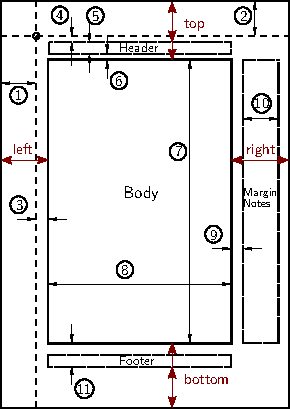
\includegraphics[scale=1.1]{./img/layout.pdf} \end{center}
	\begin{tabular}{ll@{\quad}ll}
		\textcircled{1} & 1in + \code?\hoffset? & \textcircled{2} & 1in + \code?\voffset?\\
		\textcircled{3} & \code?\oddsidemargin? & \textcircled{4} & \code?\topmargin?\\
		\textcircled{5} & \code?\headheight? & \textcircled{6} & \code?\headsep?\\
		\textcircled{7} & \code?\textheight? & \textcircled{8} & \code?\textwidth?\\
		\textcircled{9} & \code?\marginparwidth? & \textcircled{10} & \code?\marginparwidth?\\
		\textcircled{11} & \code?\footskip? \\
	\end{tabular}	

	Additional paramter: \code?left,right,top,bottom?, \code?paper=a4paper?, \code?landscape|portrait?, \code?includehead,includefoot?, \code?twocolumn?
}


\sectionbox{
	\subsection{Header and Footer with \code{fancyhdr}}
\begin{lstlisting}
\usepackage{fancyhdr}
\pagestyle{fancy}		% use fancyhdr pagestyle
\fancyhf{}					% clear header and footer
\fancyhead[RE]{}    % even page right header
\end{lstlisting}
}


\sectionbox{
	\subsection{Colors with \code?xcolor?}
\begin{lstlisting}
\usepackage{xcolor}	
\definecolor{tum_blue}{RGB}{0, 115, 207}
\colorlet{col_section}{tum_blue}
\end{lstlisting}
Predefined colors:\\ 
\texttt{white, \textcolor{gray}{gray}, black, \textcolor{red}{red}, \textcolor{green}{green}, \textcolor{blue}{blue}, \textcolor{cyan}{cyan}, \textcolor{magenta}{magenta}, \textcolor{yellow}{yellow}}\\
Fade a color with \code?!value? between 0 and 100, e.g. \code?\color{gray!70}?\\
Usage in Text: \code?\textcolor{red}{text}? or \code?{\color{red}text}?
}

\columnbreak

% SECTION ====================================================================================
\section{Structure the Document}
% ============================================================================================

\sectionbox{
	\subsection{Title with \code?titlepage?}
	default: \code!\author{!\textit{text}\code!}!, \code!\title{!\textit{text}\code!}!, \code!\date{\today}!, \qquad \code?\maketitle?\\
	titlepage: \code?\begin{titlepage}? \textit{text} \code?\end{titlepage}?
}

\sectionbox{
	\subsection{Table of Content, List of \ldots}
	\code!\tableofcontents! \qquad \code!\listoftables! \qquad \code!\listoffigures!\\
	\code?\printglossaries? (needs \code?glossaries? package) 
}


\sectionbox{
	\subsection{Headings}
	\begin{tabular}{l@{\qquad\qquad}l}
	\code!\part{!\textit{title}\code!}!  & \code!\subsubsection{!\textit{title}\code!}!  \\
	\code!\chapter{!\textit{title}\code!}! & \code!\paragraph{!\textit{title}\code!}!  \\
	\code!\section{!\textit{title}\code!}! & \code!\subparagraph{!\textit{title}\code!}! \\
	\code!\subsection{!\textit{title}\code!}!  \\
	\end{tabular}

	*: no numbering, no entry in ToC\\
	\code?\part? and \code?\chapter? only in dcumentcalss \code?book? or \code?report? 
}

\sectionbox{
\subsection{Lists}
\code?\begin{itemize}? with bullet \code?\item? \qquad or \code?\item[?\textit{symbol}\code?]?\\
\code?\begin{enumerate}? with numbered \code?\item?\\
\code?\begin{description}? with bold \code?\item[word]?
\begin{lstlisting}
\begin{enumerate}\itemsep0pt
	\item First Argument
	\item Second Argument
\end{enumerate}
\end{lstlisting}
}




% SECTION ====================================================================================
\section{Text}
% ============================================================================================

\sectionbox{
	\subsection{Fonts}
	\begin{tabular*}{\columnwidth}{l@{\extracolsep\fill}ll} \trule
	\textsc{Command} & \textsc{Declaration} & \textsc{Effect} \\ \mrule
	\code!\textrm{!\textit{text}\code!}!                    & %
			\code!{\rmfamily !\textit{text}\code!}!               & %
			\textrm{Roman family} \\
	\code!\textsf{!\textit{text}\code!}!                    & %
			\code!{\sffamily !\textit{text}\code!}!               & %
			\textsf{Sans serif family} \\
	\code!\texttt{!\textit{text}\code!}!                    & %
			\code!{\ttfamily !\textit{text}\code!}!               & %
			\texttt{Typewriter family} \\
	\code!\textmd{!\textit{text}\code!}!                    & %
			\code!{\mdseries !\textit{text}\code!}!               & %
			\textmd{Medium series} \\
	\code!\textbf{!\textit{text}\code!}!                    & %
			\code!{\bfseries !\textit{text}\code!}!               & %
			\textbf{Bold series} \\
	\code!\textup{!\textit{text}\code!}!                    & %
			\code!{\upshape !\textit{text}\code!}!               & %
			\textup{Upright shape} \\
	\code!\textit{!\textit{text}\code!}!                    & %
			\code!{\itshape !\textit{text}\code!}!               & %
			\textit{Italic shape} \\
	\code!\textsl{!\textit{text}\code!}!                    & %
			\code!{\slshape !\textit{text}\code!}!               & %
			\textsl{Slanted shape} \\
	\code!\textsc{!\textit{text}\code!}!                    & %
			\code!{\scshape !\textit{text}\code!}!               & %
			\textsc{Small Caps shape} \\
	\code!\emph{!\textit{text}\code!}!                      & %
			\code!{\em !\textit{text}\code!}!               & %
			\emph{Emphasized} \\
	\code!\textnormal{!\textit{text}\code!}!                & %
			\code!{\normalfont !\textit{text}\code!}!       & %
			\textnormal{Document font} \\
	\code!\underline{!\textit{text}\code!}!                 & %
															& %
			\underline{Underline}\\ \brule
	\end{tabular*}
}


\sectionbox{
	\subsection{Font size}
	\begin{tabular}{ll}
	\code!\tiny!                  &  \tiny{tiny} \\
	\code!\scriptsize!            &  \scriptsize{scriptsize} \\
	\code!\footnotesize!          &  \footnotesize{footnotesize} \\
	\code!\small!                 &  \small{small} \\
	\code!\normalsize!            &  \normalsize{normalsize} \\
	\code!\large!                 &  \large{large}
	\end{tabular} \qquad	
	\begin{tabular}{ll}	
	\code!\Large!                 &  \Large{Large} \\  % Tab hack for new column
	\code!\LARGE!                 &  \LARGE{LARGE} \\
	\code!\huge!                  &  \huge{huge} \\
	\code!\Huge!                  &  \Huge{Huge}
	\end{tabular}
}

\sectionbox{
	\subsection{Justification}
	\begin{tabular}{@{}lll@{}}
	\textsc{Environment}  &  \textsc{Declaration} & \textsc{Other} \\
	\code!\begin{center}!      & \code!\centering! & \textit{text} \code?\vfill? \textit{text}\\
	\code!\begin{flushleft}!  & \code!\raggedright! & \textit{text} \code?\hfill? \textit{text}\\
	\code!\begin{flushright}! & \code!\raggedleft!  \\
	\end{tabular}
}

\columnbreak

% SECTION ====================================================================================
\section{Math Equations}
% ============================================================================================
\sectionbox{
	Textstyle: \code!$x^2 + 4$!, $x^2 + 4$ as part of the text.\\
	Disyplaystyle: \code!\begin{equation} x^2 + 4 \end{equation}!\\
	\begin{equation}
			\lambda := \lim\limits_{x_1 \rightarrow \infty}    \int\limits_{x_0}^{x_1} \frac{ f\left(\frac{t}{2}\right) }{ \sqrt[n]{t^2 + \sin^2(t) } } \; \mathrm dt \stackrel{!}\le 1
	\end{equation}
	for numbered equations. use the * variant for unnumbered equations.
}


\sectionbox{
	\subsection{Fonts and Sizes in Math Mode}
	\code?\scriptscriptstyle, \scriptstyle, \textstyle, \displaystyle?\\
	\code?\mathrm, \mathit, \mathbb, \mathcal, \mathfrak?
}

\sectionbox{
	\subsection{Often used math expressions}
	\renewcommand{\arraystretch}{1.5}
	\everymath{\displaystyle}
	\begin{tabular}{@{}ll@{\qquad\quad}ll@{}}
		$x^{n+1}$ & \code#x^{n+1}# & $E_{\mathrm{kin}}$ & \code#E_{\mathrm{kin}}# \\
			
		$\frac{a+b}{2}$ & \code#\frac{a+b}{2}# & $\sqrt[n]{a^2+b^2}$ & \code#\sqrt[n]{a^2+b^2}#\\
	\end{tabular}

	\begin{tabular}{@{}lm{4cm}@{}}
		$x_1 , \ldots, x_n$ & \code#x_1 , \ldots, x_n# \\
		$x_1 + \cdots + x_n$ & \code#x_1 + \cdots + x_n#\\	
		$\left( a + \frac12 \right)^2$ & \code#\left( a + \frac12 \right)^2#\\ 
		$\sum\limits_{i=1}^{N}, \prod\limits_{i=1}^{N}$ & \code#\sum\limits_{i=1}^{N},# \newline \code#\prod\limits_{i=1}^{N}#\\
		$\vec F_{\perp}, \vec F_{\parallel}$ & \code#\vec F_{\perp}#, \code#\vec F_{\parallel}#\\
		$\lim\limits_{a \rightarrow \infty}$ & \code#\lim\limits_{a \rightarrow \infty}#\\ 
		$\int\limits_a^b x^2\; \mathrm{d}x$ & \code#\int\limits_a^b x^2\; \mathrm{d}x#\\
		$\left.\frac{\mathrm df}{\mathrm dx} \right|_{x_0}$ & \code#\left.\frac{\mathrm df}{\mathrm dx}# \code#\right|_{x_0}#\\
		$\vec a^\top, A^\dagger, A^*$ & \code#\vec a^\top, A^\dagger, A^*#\\ 
		$\stackrel{!}{<}, \stackrel{\rm def}{=}$ & \code#\stackrel{!}{<}, \stackrel{\rm def}{=}#\\
		%$\overset{oben}{mitte}, \underset{unten}{mitte}$ & \code#\overset{oben}{mitte}, \underset{unten}{mitte}#\\
	\end{tabular} 
	\everymath{\textstyle}		
}


\sectionbox{
	\subsection{Math function names (upright, correct spacing)}
	\begin{tabular}{@{}llllllll}
	\code?\sin? & \code?\sinh? & \code?\arcsin? & \code?\csc? & \code?\ln? & \code?\min?\\
	\code?\cos? & \code?\cosh? & \code?\arccos? & \code?\sec? & \code?\lg? & \code?\max?\\
	\code?\tan? & \code?\tanh? & \code?\arctan? & \code?\cot? & \code?\log? & \code?\lim?\\
	\code?\exp? & \code?\det? & \code?\tr? & \code?\dim? & \code?\ker? & \code?\Pr?\\
	\end{tabular}
}

\sectionbox{
	\subsection{Important Math functions}
	\begin{tabular}{@{}llllllllll}
	$\sum$ & \code?\sum? & $\prod$ & \code?\prod? & $\int$ & \code?\int?\\
	$\int$ & \code?\int? & $\iint$ & \code?\iint? & $\iiint$ & \code?\iiint? & $\oint$ & \code?\oint?\\
	$\vec a$ & \code?\vec a? & $\dot a$ & \code?\dot a? & $\ddot a$ & \code?\ddot a? & $\hat a$ & \code?\hat a? \\
	\end{tabular}
}

\sectionbox{
	\subsection{Important Symbols in Mathmode}
	\tabcolsep=4pt

	\begin{tabular}{@{}cl@{\hspace{2em}}cl@{\hspace{2em}}cl@{\hspace{2em}}cl}
	$+$ & \code?+? & $-$ & \code?-? & $\pm$ & \code?\pm? & $\mp$ & \code?\mp?\\
	$<$ & \code?<? & $\le$ & \code?\le? & $\ll$ & \code?\ll? & $\cdot$ & \code?\cdot?\\
	$>$ & \code?>? & $\ge$ & \code?\ge? & $\gg$ & \code?\gg? & $\times$ & \code?\times?\\
	$=$ & \code?=? & $\ne$ & \code?\ne? & $\equiv$ & \code?\equiv? & $\approx$ & \code?\approx?\\
	$|$ & \code?|? & $\perp$ & \code?\perp? & $\mid$ & \code?\mid? & $\parallel$ & \code?\parallel?\\
	$f'$ & \code?f'? & $\nabla$ & \code?\nabla? & $\Delta$ & \code?\Delta? & $\partial$ & \code?\partial?\\
	$\in$ & \code?\in? & $\forall$ & \code?\forall? & $\exists$ & \code?\exists? & $\nexists$ & \code?\nexists?\\
	$\cap$ & \code?\cap? & $\cup$ & \code?\cup? & $\notin$ & \code?\notin? & $\setminus$ & \code?\setminus?\\
	$\ell$ & \code?\ell? & $\angle$ & \code?\angle? & $\circ$ & \code?\circ? & $\emptyset$ & \code?\emptyset?\\
	$\lor$ & \code?\lor? & $\land$ & \code?\land? & $\lnot$ & \code?\lnot? & $\varnothing$ & \code?\varnothing?\\
	$\top$ & \code?\top? & $\bot$ & \code?\bot? & $\infty$ & \code?\infty? & $\propto$ & \code?\propto?\\
	\end{tabular}
}

\sectionbox{
	\subsection{Delimeters}
	\tabcolsep=3pt
	\begin{tabular}{@{}cl@{\hspace{3em}}cl@{\hspace{3em}}cl@{\hspace{2em}}cl}
	$(.)$ & \code?(.)? & $[.]$ & \code?[.]? & $\lfloor.\rfloor$ & \code?\lfloor.\rfloor?\\
	$|.|$ & \code?|.|? & $\{.\}$ & \code?\{.\}? & $\lceil.\rceil$ & \code?\lceil.\rceil?\\
	$\|.\|$ & \code?\|.\|? & $\vert.\vert$ & \code?\vert.\vert? & $\langle.\rangle$ & \code?\langle.\rangle?\\
	\end{tabular}	

	Use \code?\left(? \textit{expr} \code?\right)? to stretch any delimeter to the height of \textit{expr}
	Or \code?\big, \Big, \bigg? for manual sizing e.g. \code?\Big\| \Big\|?
}

\sectionbox{
	\subsection{Arrows}
	Every combination of left,right,up,down with arrow(s)\\
	\begin{tabular}{@{}llll}
	$\mapsto$ & \code?\mapsto? & $\leadsto$ & \code?\leadsto?\\
	$\rightarrow$ & \code?\rightarrow? & $\Rightarrow$ & \code?\Rightarrow?\\
	$\longrightarrow$ & \code?\longrightarrow? & $\Longrightarrow$ & \code?\Longrightarrow?\\
	$\leftarrow$ & \code?\leftarrow? & $\Leftarrow$ & \code?\Leftarrow?\\
	$\longleftarrow$ & \code?\longleftarrow? & $\Longleftarrow$ & \code?\Longleftarrow?\\
	$\uparrow$ & \code?\uparrow? & $\Uparrow$ & \code?\Uparrow?\\
	$\downarrow$ & \code?\downarrow? & $\Downarrow$ & \code?\Downarrow?\\
	$\leftrightarrow$ & \code?\leftrightarrow? & $\Leftrightarrow$ & \code?\Leftrightarrow?\\
	$\leftleftarrows$ & \code?\leftleftarrows? & $\rightrightarrows$ & \code?\rightrightarrows?\\
	$\leftrightarrows$ & \code?\leftrightarrows? & $\rightleftarrows$ & \code?\rightleftarrows?\\
	$\leftrightharpoons$ & \code?\leftrightharpoons? & $\rightleftharpoons$ & \code?\rightleftharpoons?\\
	\end{tabular}	
}

\sectionbox{
	\subsection{Physical Units with \code?siunitx?}
	\sisetup{sticky-per=true}
	\sisetup{per-mode=reciprocal}
	Use the package \code#siunitx# for correct display of numbers and units. It provide the commands \code#\num{<number>}#, \code#\si{<unit>}#, and \code#\SI{<number>}{<unit>}#. Some examples:\\
	
	\begin{tabular}{@{}ll@{}}
	$\num{7.123456e12}$ & \code#\num{7.123456e12}#\\[0.5em]
	$[g] = \si{\meter \per \second \squared}$ & \code#[g] = \si{\meter \per \second \squared}#\\[0.5em]
	$E = \SI[per-mode=fraction]{1.3}{\kilo\volt\per\milli\meter}$ & \code#E = \SI{1.3}{\kilo\volt\per\milli\meter}#\\
	\end{tabular}\\
	\\
	You can use all SI units (pascal, henry, ...) and not only the base units. It is also possible to change the style of display with
	\code#\sisetup{per-mode=reciprocal}# or \code#\sisetup{per-mode=fraction}#:\\
	Prefixes like \code?\kilo,\deca,\mega,\micro?
}


% SECTION ====================================================================================
\section{LaTeX4EI classes \& packages}
% ============================================================================================
\sectionbox{
	\code?latex4ei_thesis:? layout with TUM colors\\
	\code?scientific:? useful scientific macros

	\begin{tabular}{ll@{\qquad\quad}ll}
	$\diff x$ & \code#\diff x# & $\N, \R, \C$ & \code#\N, \R, \C# \\
	$\vec x$ & \code?\vec x? & $\vect{ x_1 \\ x_2 }$ & \code#\vect{ x_1 \\ x_2 }#\\[2em]
	$\ma A$ & \code#\ma A# & $\mat{ 1 & 2 \\ 3 & 4}$ & \code#\mat{ 1 & 2 \\ 3 & 4}#\\[2em]
	$\FT$ & \code#\FT# & $\DTFT$ & \code#\DTFT#\\
	$\LT$ & \code#\LT# & $\ZT$ & \code#\ZT#\\
	\end{tabular}
	% norm{} \unitof{}

	Additional function names (upright, correct spacing):\\ \code?\const, \sinc, \grad, \rot, \div, \tri, \rect, \erf?
}



% SECTION ====================================================================================
\section{Floating Environments}
% ============================================================================================

\sectionbox{
	\subsection{Figures with \code?graphicx?}
	\begin{lstlisting}
\begin{figure}
	\centering
	\includegraphics[width=9cm]{./img/diagram.pdf}
	\caption[title for LOF]{this is the long title}
	\label{fig:example1}
\end{figure}
	\end{lstlisting}

	Load image: \code!\includegraphics[width=!\textit{x}\code!]{!\textit{file}\code!}!\\
	Alter numbering: \code?\renewcommand\thefigure{\arabic{figure}}?

		\subsubsection{Subfigures with \code?subfigure?}
		Usage \code?\subfigure[?\textit{caption}\code?]{?\textit{graphic, label}\code?}?
}

\sectionbox{
\subsection{Tables}
\begin{lstlisting}
\begin{table}
	\centering
	\begin{tabular}{ll} 
		\textsc{Name} & \textsc{Desc.}\\ \hline
		test1 & is no good idea &\\
		bla2 & even worse &\\ 
	\end{tabular}
	\caption{My first Table}
	\label{tab:example1}
\end{table}
\end{lstlisting}

Usage: \code?\begin{tabular}[htbp]{@{}lrc|p{3cm}}?\\
Column distance: \code?\setlength{\tabcolsep}{5pt}?\\
Adjust row distance: \code?\renewcommand{\arraystretch}{1.5}?\\			%\tabularnewline
Partial lines: \code?\cline{2-3}? instead of \code?\hline?\\
Additional packages: \code?longtable, booktabs, colortbl?
}

\sectionbox{
\subsection{Source Code Listings with \code?listings?}
Options: \code?\lstset{basicstyle=\tt, language=C}?\\
Languages: C,C++,Java,Matlab,Python,HTML,XML,bash,...\\[1em]
Environment: \code?\begin{lstlisting}? \textit{code} \code?\end{lstlisting}?\\
Inline: \code+\lstinline?+\textit{code}\code+?+\\
\lstset{language=Java}
\begin{lstlisting}
\begin{lstlisting}
int i=0;
for(i = 0; i < 10; i++){
	printf("Line %i", i);
}
\end{ltlisting}		% missing s!
\end{lstlisting}
}
\lstset{language={[LaTeX]TeX}}



% SECTION ====================================================================================
\section{Correct Typography}
% ============================================================================================



\sectionbox{
	\subsection{Hyphen and Dashes}
	Rule: The hyphen is never placed between two spaces!\\
	\begin{tabular*}{\columnwidth}{l@{\extracolsep\fill}lll} \trule
	\textsc{Name} & \textsc{Source} & \textsc{Example} & \textsc{Usage} \\ \mrule
	hyphen  & \code!-!   & X-ray, in- and output  & connect words\\
	en-dash & \code!--!  & 1 -- 5, Paris -- Rom & seperate numbers. \\
	em-dash & \code!---! & Yes---or no?    & Punctuation.\\
	minus & \code!$-$! & $5 - 3 = 2$ & Equations.\\ \brule
	\end{tabular*}
}

\sectionbox{
	\subsection{Quotation Marks}
	\begin{tabular*}{\columnwidth}{l@{\extracolsep\fill}ll} \trule
		\textsc{Language} & \textsc{Symbols} & \textsc{LaTeX}\\ \mrule
		German & \glqq\ \glq\ …\ \grq\ \grqq & \code?\glqq \glq ... \grq \grqq?\\
		English & ``\ \lq\ …\ \rq\ " & \code?`` \lq ... \rq ''?\\
		France & \flqq \flq … \frq \frqq & \code?\flqq \flq ... \frq \frqq?\\ \brule
	\end{tabular*}
	
	“I think”, said Anna, “he shouted ‘This is Lars’s car!’, when I saw him.”
}

\sectionbox{
	\subsection{Numbers and Dates}
	\begin{tabular}{lll}
	\textsc{Numbers} & \textsc{Look} & \textsc{Usage}\\ \mrule
	old-style & \oldstylenums{1234567890} & as part of text, dates\\
	lining & $1234567890$ & as math value\\
	\end{tabular}

	\vspace{1em}
	
	\begin{tabular}{lll}
		\textsc{British} & \textsc{American} & \textsc{German}\\ \mrule
		27/06/93 & 06/27/93 & 27.06.1993\\
		27 June, 1993 & June 27, 1993 & 27. Juni 1993\\
	\end{tabular}
	
	International notation (ISO 8601): yyyy-mm-dd: 1993-06-27
}

\sectionbox{
	\subsection{Spacing}
	\setlength{\tabcolsep}{6pt}
	\begin{tabular}{@{}ll|ll|ll|ll} 
		\code?a\!b? & a\!b & \code?a\,b? & a\,b & \code?a\;b? & a\;b & \code?a\quad b? & a\quad b\\
		\code?ab? & ab & \code?a\>b? & a$\>$b & \code?a\ b? & a\ b & \code?a\qquad b? & a\qquad b\\
	\end{tabular}

	\code?\hspace{?\textit{length}\code?}?, \code?\vspace{?\textit{length}\code?}? \qquad *: even at line start\\
	\code?\phantom{?\textit{text}\code?}?, \code?\vphantom{?\textit{text}\code?}?\\
	Protected space \code?~?
}

\sectionbox{
	\subsection{Boxes and Rules}
	Normal: \code?\parbox[pos][height][contentpos]{width}{text}? or\\
	\code?\begin{minipage}[pos][height][contentpos]{width} text?\\
	\\
	Prevent line breaking: \code?\mbox{text}?\\
	Lift Text: \code?\raisebox{lift}[height][depth]{text}?\\
	Framed Box: \code?\framebox[width][pos]{text}? or \code?\fbox{text}?\\
	Resize: \code?\scalebox{10}{Giant}?\\
	Lengths: \code?\setlength{\fboxsep}{10pt}, \setlength{\fboxrule}{2pt}?
}



% SECTION ====================================================================================
\section{Bibliography with \BibTeX}
% ============================================================================================

\renewcommand{\arraystretch}{1.2}

\sectionbox{
	\subsection{\BibTeX\ entry types}
	\begin{tabular}{ll}
		\code!@article!         &  Journal or magazine article. \\
								& fields: \code!author, title, journal, year, volume!\\[0.5em]
		\code!@book!            &  Book with publisher. \\
								& fields: \code!author/editor, title, publisher, year!\\[0.5em]
		\code!@techreport!      &  Tech report, usually numbered in series. \\
								& fields: \code!author, title, institution, year!\\[0.5em]
		\code!@phdthesis!       &  PhD. or other thesis. \\
								& fields: \code!author, title, school, year!\\
	\end{tabular}

\begin{lstlisting}
\bibliographystyle{alphadin}
\bibliography{<bibliographyfile.bib>}
\end{lstlisting}	
}


\sectionbox{
	\subsection{References with \code?hyperref?}
	\begin{tabular}{@{}lp{4cm}@{}}
	\code!\cite{!\textit{key}\code!}! & Cite a reference\\
	\code!\label{!\textit{marker}\code!}!   &  Set a marker for cross-reference, 
	                          often of the form \code!\label{sec:item}! like \code?\label{fig:diag1}?. \\
	\code!\ref{!\textit{marker}\code!}!   &  Give section/body number of marker. \\
	\code!\pageref{!\textit{marker}\code!}! &  Give page number of marker. \\
	\code!\footnote{!\textit{text}\code!}!  &  Print footnote at bottom of page. \\
	\code?\url{?\textit{url}\code?}? & Creates click-able web-adress.\\
	\code?\href[?\textit{options}\code?]{?\textit{url}\code?}{?\textit{text}\code?}? & click-able link\\
	\code?\hyperref[?\textit{marker}\code?]{?\textit{text}\code?}? & click-able ref\\
	\end{tabular}
}

\subsection{Reference management software supporting \BibTeX}
\href{http://www.mendeley.com/}{Mendeley}: free, Win/Linux/Mac, import from several websites\\
\href{http://www.citavi.com}{Citavi}: free, Win



% SECTION ====================================================================================
\section{Include beautiful Matlab Plots}
% ============================================================================================
Same font, line width, vector graphic




% SECTION ====================================================================================
\section{Own Commands and Writing Packages}
% ============================================================================================
\sectionbox{
	\begin{tabular}{ll}
		\code?\usepackage[?options\code?]{?package\code?}? & load package\\
		\code?\newcommand[?paranum\code?]{\newcmd}{?tex \#1\code?}? & define command\\
		\code?\renewcommand{\cmd}{? latex \#1,\#2 \code?}? & alter command\\
		\code?\let\cmdcopy\cmd? & copy a command\\ 
	\end{tabular}

Read this document CTAN\\

Some important variables:\\
Counters: \code?\thepage, \thesection, \thefigure?\\
Lengths: \code?\textwidth, \parindent, \parskip?\\
}

\sectionbox{
	\subsection{Plain \TeX}
	These plain \TeX~commands should be used carefully\\
	\begin{tabular}{lll}
	Fonts & \code?\rm, \sf, \sc, \sl, \it, \tt?\\
	Definitions & \code?\def\newcmd{?texcode\code?}, \let\newcmd\cmd?\\
	If & \code?\ifnum\counter<10? true text \code?\else? false text \code?\fi?\\
	\end{tabular}
}

% SECTION ====================================================================================
\section{Useful Weblinks}
% ============================================================================================
\sectionbox{
	\begin{tabular}{ll}
	LaTeX4EI & \url{www.latex4ei.de}\\
	Font \& Symbols & \url{https://de.wikipedia.org/wiki/Hilfe:TeX}\\
	Color Schemes & \url{http://colorschemedesigner.com}\\
	\end{tabular}


	Tipps for Package Writers: %\url{latex-project.org/guides/clsguide.pdf‎}
}
% Ende der Spalten
\end{multicols*}

% Dokumentende
% ======================================================================
\end{document}



	\subsection{Modify Headings with \code?titlesec?}
	\code?\titleformat{?\textit{cmd}\code?}[?\textit{shape}\code?]{?\textit{format}\code?}{?\textit{label}\code?}{?\textit{sep}\code?}{?\textit{before}\code?}[?\textit{after}\code?]?\\
	\code?\titlespacing*{ command }{ left }{ before-sep }{ after-sep }[ right-sep ]?




\sectionbox{
	\subsection{Font Combinations}
	Rule: Use serif fonts for long body text and sans-serif for headings!\\
	\begin{tabular}{lll} \trule
	\textsc{Serif} & \textsc{Sans} & \textsc{Mono}\\ \mrule
	\textrm{Computer Modern} & \textsf{Computer Modern} & \texttt{Computer Modern}\\
	Cambria & Calibri & Consolas\\
	Palantino & Bera & Bera\\
	Minion & Myriad & \\ \brule
	\end{tabular}
}







